\documentclass[12pt,a4paper,openright,twoside]{book}
\usepackage[utf8]{inputenc}
\usepackage{disi-thesis}
\usepackage{code-lstlistings}
\usepackage{notes}
\usepackage{shortcuts}
\usepackage{acronym}
\usepackage{listings}
\usepackage{xcolor}
\usepackage{tikz}

\lstdefinelanguage{json}{
    basicstyle=\footnotesize\ttfamily,
    numbers=left,
    numberstyle=\tiny,
    breaklines=true,
    frame=lines,
    backgroundcolor=\color{gray!10},
    showstringspaces=false,
    string=[db]{"},
    stringstyle=\color{green!50!black},
    morestring=[s][\color{black}]{\ \ "}{":},
    keywordstyle=\color{blue},
    keywords={true,false,null},
    literate=
     *{0}{{{\color{red}0}}}{1}
      {1}{{{\color{red}1}}}{1}
      {2}{{{\color{red}2}}}{1}
      {3}{{{\color{red}3}}}{1}
      {4}{{{\color{red}4}}}{1}
      {5}{{{\color{red}5}}}{1}
      {6}{{{\color{red}6}}}{1}
      {7}{{{\color{red}7}}}{1}
      {8}{{{\color{red}8}}}{1}
      {9}{{{\color{red}9}}}{1}
      {.}{{{\color{red}.}}}{1}
      {:}{{{\color{gray}{:}}}}{1}
      {,}{{{\color{gray}{,}}}}{1}
      {\{}{{{\color{gray}{\{}}}}{1}
      {\}}{{{\color{gray}{\}}}}}{1}
      {[}{{{\color{gray}{[}}}}{1}
      {]}{{{\color{gray}{]}}}}{1},
}

\usetikzlibrary{shapes,arrows,positioning}
\usetikzlibrary{fit}
\usetikzlibrary{calc}
\tikzstyle{block} = [rectangle, draw, fill=white, 
    text width=3cm, text centered, rounded corners, minimum height=2em]
\tikzstyle{line} = [draw, -latex']

\school{\unibo}
\programme{Corso di Laurea in Ingegneria e Scienze Informatiche}
\title{Integrazione di RAG e LLM nello Sviluppo del Software}
\author{Bollini Simone}
\date{\today}
\subject{Programmazione ad oggetti}
\supervisor{Prof. Viroli Mirko}
\cosupervisor{Dott. Aguzzi Gianluca}
%\morecosupervisor{Dott. Farabegoli Nicolas}
\session{IV}
\academicyear{2023-2024}

% Definition of acronyms
\acrodef{RAG}{Retrieval-Augmented Generation}
\acrodef{AI}{Artificial intelligence}
\acrodef{LLM}{Large Language Model}


\mainlinespacing{1.241} % line spacing in mainmatter, comment to default (1)

\begin{document}

\frontmatter \frontispiece

\begin{abstract}	
I \ac{LLM} addestrati per sviluppare il codice sono oggi altamente efficaci e in grado di generare soluzioni di qualità.
L'addestramento fatto sui modelli è però su fonti generali, questo non da quindi la possibilità al modello di generare soluzioni su misura per una specifica richiesta utilizzando codice già creato dal programmatore o dalla propria azienda per casi simili.
Da questo nasce l'esigenza di addestrare il modello per personalizzare le soluzioni proposte, contestualizzandole alla propria realtà aziendale e al proprio stile nel programmare ma
il fine-tuning di un \ac{LLM} è un processo molto costoso e difficile da utilizzare per mantenere aggiornato frequentemente la base di conoscenza del modello.
Per rispondere a questa esigenza entra in gioco la \ac{RAG}, che permette di aumentare la conoscenza del modello, recuperando informazioni da una propria base di conoscenza, esterna al modello, come librerie specifiche di un azienda, arricchendo il prompt della query di input che sarà elaborata dal LLM.
Il \ac{RAG}, ricercando semanticamente i chunk maggiormente somiglianti a quanto richiesto se trovati, li inserirà per aumentare il prompt del LLM, estendendo la base di informazioni sulla quale genererà l'output con la risposta.
Questa tesi approfondisce questi concetti e sperimenta l'integrazione di un \ac{RAG} specifico per codice Java e un \ac{LLM} con lo scopo di ottenere dal LLM risposte personalizzate
che solo con la conoscenza del LLM, anche se estremamente performante e completo, sarebbe stato impossibile ottenere.
\end{abstract}

\begin{dedication}
A Giulia e ai miei figli, il dono più grande.
\newline A tutta la mia famiglia.
\newline Grazie a tutti voi.
\end{dedication}

%----------------------------------------------------------------------------------------
\tableofcontents   
%\listoffigures     % (optional) comment if empty
%\lstlistoflistings % (optional) comment if empty
%----------------------------------------------------------------------------------------

\mainmatter

%----------------------------------------------------------------------------------------
\chapter{Introduzione}
\label{chap:introduction}
%----------------------------------------------------------------------------------------

\section{Essere programmatori nel 2025}
Per sviluppare codice sono disponibili tantissimi (IDE), uno di questi è \textbf{Visual Studio Code},
mentre per condividere i progetti e lavorare in team lo strumento utilizzato potrebbe essere  \textbf{GitHub}.
Se richiesta memoria GPU per piccoli progetti accademici è disponibile ad esmpio \textbf{COLAB}, che permette di eseguire in remoto codice utilizzando GPU senza costi.
Questi esempi sono parte di una panoramica di strumenti sempre più vasta, complessa e in rapita evoluzione, con un frequente cambio di software per realizzare un programma.
Inoltre i possibili modi per realizzare i progetti è aumentanta, disponendo oggi di sempre più librerie e metodi per realizzare il codice.
Un esempio d'utilizzo degli strumenti sopra elencati potrebbe seguire la seguente scaletta:
\begin{itemize}
    \item Realizzazione iniziale del progetto in locale utilizzado Visual Studio Code
    \item Push del codice su GitHub per condividere il progetto con il team
    \item Esecuzione del codice su Colab per testare il codice su GPU ed eventualmente eseguire modifiche concluse con nuovo Push su GitHub
    \item Pull in locale per continuare a lavorare sul progetto
\end{itemize}
Questo modo dinamico di lavorare è recente ma non una novità, come invece lo sono alcuni specifici strumenti forniti da questi software tutti accumunati \textbf{dall'implementazione al loro interno di funzioni basate sull'IA}.
Queste funzioni sono in grado di completare il codice, suggerire correzioni e creare documentazione pertinente.
GitHub ha introdotto \textbf{Copilot}, un assistente IA per la scrittura del codice, questo strumento è integrabile per vari IDE tra cui proprio Visual Studo Code.
Un esempio semplice ma che offre già un idea della vastità e della potenza di queste funzioni è l'utility di \textbf{Github Copilot} 'Generate Commit Message with Copilot'
che propone il testo da utilizzare come descrizione di un commit, ho provato a riscontrare quanto fosse contestualizzato e coerente 
con quanto aggiornato e ho ottenuto il seguente risultato:
\begin{figure}[h]
    \centering
    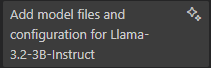
\includegraphics[width=0.5\linewidth]{figures/commit.png}
    \label{fig:Commit-Autogenerato}
\end{figure}
\newline
Nel mio caso quanto proposto era corretto ed ho quindi eseguito il Commit con la descrizione proposta.
Quanto è riuscito a fare Copilot è strabiliante, in pochi istanti ha analizzato il contesto ritornando come output una risposta semplice ma coerente rispetto a quanto cambiato.
L'uso di questi strumenti sta rendendo il lavoro molto più dinamico e veloce, riducendo le interruzioni nel cercare soluzioni o per trovare le giuste parole per descrivere
quanto fatto.
\begin{figure}[h]
    \centering
    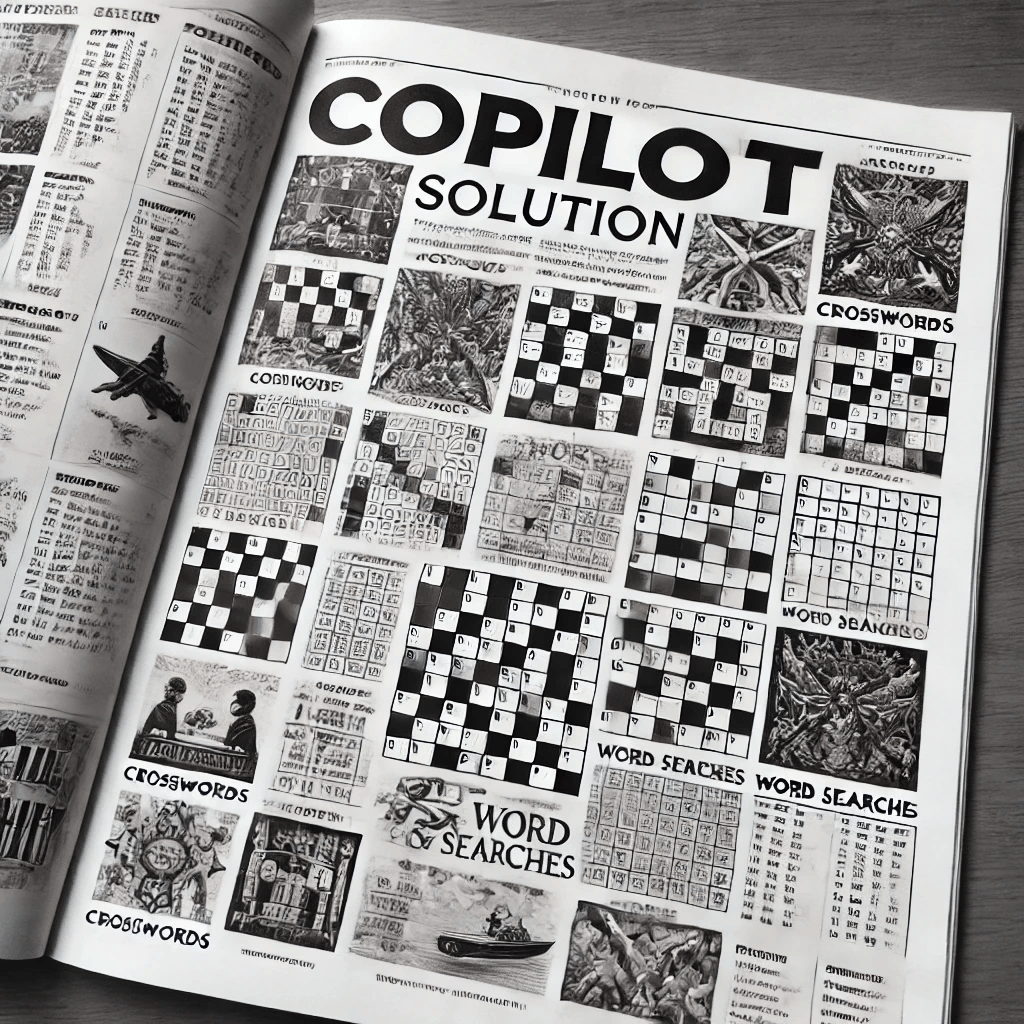
\includegraphics[width=0.5\linewidth]{figures/copilotsolutionSettimanaEnigmistica.png}
    \label{fig:Copilot-Solution}
\end{figure}
\newline
L'intelligenza artificiale sta rivoluzionando il modo in cui il software viene sviluppato, strumenti come Copilot utilizzando tutto il loro potenziale, possono creare la spina dorsale di un progetto
in poco tempo lasciando al programmatore il compito di verificare e correggere solo in parte il codice proposto. 
In progetti complessi questo non riduce il ruolo del programmatore, anzi lo eleva a compiti di precisione e ad alto valore aggiunto delegando la stesura di parti del codice semplici e ripetitive al software stesso.
Per questi motivi capire come funzionano oggi questi strumenti è importante, sapere come chiedere e formulare correttamente le domande al LLM è fondamentale, esplicitando nel dettaglio con parole chiave mirate come deve essere realizzato il codice per indirizzarlo nell'elaborazione e ragionamento corretto.
Altro compito complesso per il programmatore è non farsi troppo ammaliare dalle soluzioni proposte perché non sempre necessarie per quanto richiesto oppure diverse da quanto già conosciuto
 per realizzare una determinata funzione.
Questo nuovo modo di lavorare permette di conoscere nuove soluzioni ma comporta test e tempo non sempre disponibile,
il programmatore deve sempre avere il controllo del progetto, accettando generazione del codice automatica solo dove consapevole di quanto proposto e del suo impatto anche in casi di revisione e manutenzione futuri.
Il codice deve rimanere rapidamente leggibile e coerente in tutte le sue parti, far generare il codice in automatico può portare ad una perdità di coerenza e leggibilità. 
Proprio per questo l'ultimo miglio da percorrere per sfruttare questi strumenti è la personalizzazione delle risposte del LLM, per ottenere risposte rimanendo nel contesto e nello stile di quanto già realizzato e conosciuto, per fare questo entra in gioco il \textbf{Fine-Tuning} e i \textbf{RAG} che verrano ampiamente approfonditi.

\chapter{Addestrare un LLM per la Generazione del Codice}

L'addestramento di LLM per la generazione del codice di programmazione richiede una serie di passaggi complessi e costi significativi.
Conoscere questo processo, senza addentrarsi nel dettaglio, è utile per poter poi comprendere al meglio la successiva implementazione con le tecniche di \textbf{RAG}.
La procedura si divide nelle seguenti fasi:
\section{Scelta Modello}
Gli LLM utilizzano tipicamente architetture basate su trasformatori, che sono particolarmente efficaci nell'elaborazione di sequenze di dati, come il testo e il codice.
I trasformatori utilizzano meccanismi di auto-attenzione per valutare l'importanza di diversi elementi in una sequenza,
permettendo al modello di comprendere le relazioni tra parole o token.
Questa capacità è fondamentale nella generazione del codice, poiché le dipendenze tra variabili e funzioni possono estendersi su ampie sezioni del codice, richiedendo al modello di considerare un ampio contesto per trovare le risposte corrette.
L'architettura del modello scelto influenzerà in maniera decisiva tutte le successive fasi di addestramento.
È utile notare che sebbene i trasformatori siano attualmente lo standard, esistono anche altri approcci come le reti neurali ricorrenti (RNN e LSTM) e nuove tecniche in continua evoluzione come i Large Concept Models \cite{code-llm-survey-2024}.
\section{Raccolta e Preparazione dei Dataset}
La qualità e la quantità dei dati per l'addestramento è di primaria importanza per prepare un modello alla generazione di codice in maniera efficace.
È quindi essenziale utilizzare per il training codice proveniente da molteplici fonti tra cui codice sorgente, file readme, documentazione tecnica, commenti nel codice,
pagine Wiki, API e discussioni su forum specializzati in programmazione, arricchendo così il dataset con esempi pratici e ricchezza terminologica.
In rete è possibile trovare diverso materiale open source tra cui dataset già etichettati. Alcuni dataset hanno un valore altissimo,
per tutelare il costo per produrli per certi dataset è previsto il diritto d'autore.
I dati si dividono in due tipologie:
\begin{itemize}
    \item \textbf{Dati Strutturati}: seguono un formato specifico e predefinito, seguono la struttora in coppie (descrizione, codice).
    \item \textbf{Dati non Strutturati}: non sono organizzati e sono quindi più difficili da interpretare dal modello. 
\end{itemize}
\subsection{Pulizia e Pre-Processo}
La raccolta di dati va visionata con cura, se non si conosce la provenienza del codice è possibile che contenga bug o codice obsoleto che possono essere trasmessi al modello.
Con la rapida evoluzione del codice molte librerie e tecniche vengono rapidamente deprecate e superate per questo anche utilizzando i più noti modelli LLM ad oggi disponibili, può capitare di ricevere come output \textbf{codice obsoleto che risolve il quesito ma con soluzioni contenti tecniche, api e librerie deprecate o non più disponibili.}
Per questo motivo i dati raccolti devono essere quindi puliti e pre-processati per rimuovere errori e informazioni non pertinenti, garantendo così un dataset di alta qualità per l'addestramento.
\newline Il modello per poter elaborare il dataset ha bisogno che quest'ultimo venga diviso in parti più piccole chiamate token per mantenere l'integrita del dato \cite{stanford-codegen},
i token possono essere parole, parti di parole o singoli caratteri, e questa suddivisione è fondamentale per:

\begin{itemize}
    \item \textbf{Gestione del contesto}: mantenere la relazione semantica tra i diversi elementi del codice
    \item \textbf{Efficienza computazionale}: processare grandi quantità di testo in modo ottimizzato
    \item \textbf{Limitazioni del modello}: rispettare i limiti massimi di input del modello (tipicamente tra 512 e 4096 token)
    \item \textbf{Preservazione della struttura}: mantenere la struttura sintattica del codice sorgente
\end{itemize}

Ad esempio, nel codice Java, i token potrebbero includere:
\begin{itemize}
    \item Parole chiave (\texttt{public}, \texttt{class}, \texttt{static})
    \item Identificatori (nomi di variabili e metodi)
    \item Operatori e simboli (\texttt{+}, \texttt{=}, \texttt{\{}, \texttt{\}})
    \item Stringhe letterali e commenti
\end{itemize}

\section{Pre-Addestramento}
Il pre-addestramento di un LLM specializzato nella generazione di codice ha lo scopo di fornire al modello una conoscenza generale della sintassi e delle strutture logiche dei linguaggio di programmazione.
Durante questa fase il modello impare a generare codice partendo da dati non etichettati utilizzando tecniche come il \emph{language modeling} autoregressivo per insegnare al modello di predire il token successivo in una sequenza.
Questo approccio rende la generazione contestualmente e coerente di codice, sfruttando la capacità del modello di "ricordare" il contesto anche su ampie sequenze di dati.
\section{Fine-Tuning}
Il fine-tuning è la fase in cui il modello già pre-addestrato viene ulteriormente specializzato per la generazione di codice adattando e migliorando il modello per specifici domini di applicazione.
Durante questa fase, il modello affina le sue capacità attraverso dataset specializzati composti da coppie descrizione-codice, documentazione tecnica e commenti, esempi di bug-fixing e refactoring.
\textbf{Tecniche di Apprendimento}:
    \begin{itemize}
        \item \textbf{Supervisionato}: Training su coppie input-output predefinite, il modello impara a mappare input di descrizione con linguaggio naturale a output di codice corrispondente.
        \item \textbf{Per Rinforzo}: Ottimizzazione basata su feedback e metriche di qualità
        \item \textbf{Few-shot Learning}: Adattamento a nuovi contesti con pochi esempi
    \end{itemize}

\subsection{Overfitting}
Il processo di fine-tuning richiede un attento bilanciamento nell'apprendere dai dati di addestramento cercando di evitare di incorrere in overfitting.
L'overfitting si verifica quando il modello si specializza troppo sui dati di addestramento, riducendo la sua capacità di generalizzazione producendo risposte errate o incoerenti su nuovi dati.
Per evitare l'overfitting vengono utilizzati set di validazione, regolarizzazione e tecniche di dropout.

\section{Pre-Addestramento vs Fine-Tuning}
È importante comprendere la distinzione tra queste due fasi:
\subsubsection{Pre-Addestramento}
Il pre-addestramento è la fase iniziale dove il modello:
\begin{itemize}
    \item Acquisisce una comprensione \textbf{generale} del linguaggio di programmazione
    \item Viene addestrato su \textbf{grandi quantità} di codice sorgente generico
    \item Impara le strutture base e la sintassi del linguaggio
    \item Non è ancora specializzato per compiti specifici
\end{itemize}

\subsubsection{Fine-Tuning}
Il fine-tuning è invece la fase di specializzazione dove il modello:
\begin{itemize}
    \item Si adatta a un \textbf{dominio specifico} o a compiti particolari
    \item Utilizza dataset specifici e composti da dati strutturati 
\end{itemize}

\section{Valutazione e Ottimizzazione}
Una volta addestrato, il modello deve essere rigorosamente valutato utilizzando metriche specifiche per la generazione di codice, come la correttezza sintattica, la funzionalità e l'efficienza del codice prodotto.
I risultati della valutazione possono essere utilizzati per ulteriori ottimizzazioni, come aggiustamenti dei pesi del modello, modifiche all'architettura o includere dati di addestramento aggiuntivi per affrontare eventuali carenze.

\subsection{Metriche di Valutazione}
\begin{itemize}
    \item \textbf{Correttezza Sintattica}: Verifica che il codice generato sia sintatticamente corretto.
    \item \textbf{Funzionalità}: Verifica che il codice generato realizzi la funzionalità desiderata.
    \item \textbf{Efficienza}: Valuta le prestazioni del codice in termini di tempo di esecuzione e utilizzo delle risorse.
\end{itemize}

\subsection{Tecniche di Ottimizzazione}
\begin{itemize}
    \item \textbf{Aggiustamento dei Pesi}: Modifica dei pesi del modello per migliorare le prestazioni.
    \item \textbf{Modifiche all'Architettura}: Introduzione di nuove componenti o modifiche a quelle esistenti.
    \item \textbf{Integrazione di Dati Aggiuntivi}: Utilizzo di ulteriori dati di addestramento per migliorare le prestazioni.
\end{itemize}

\chapter{RAG}
\begin{figure}[h]
    \raggedright
    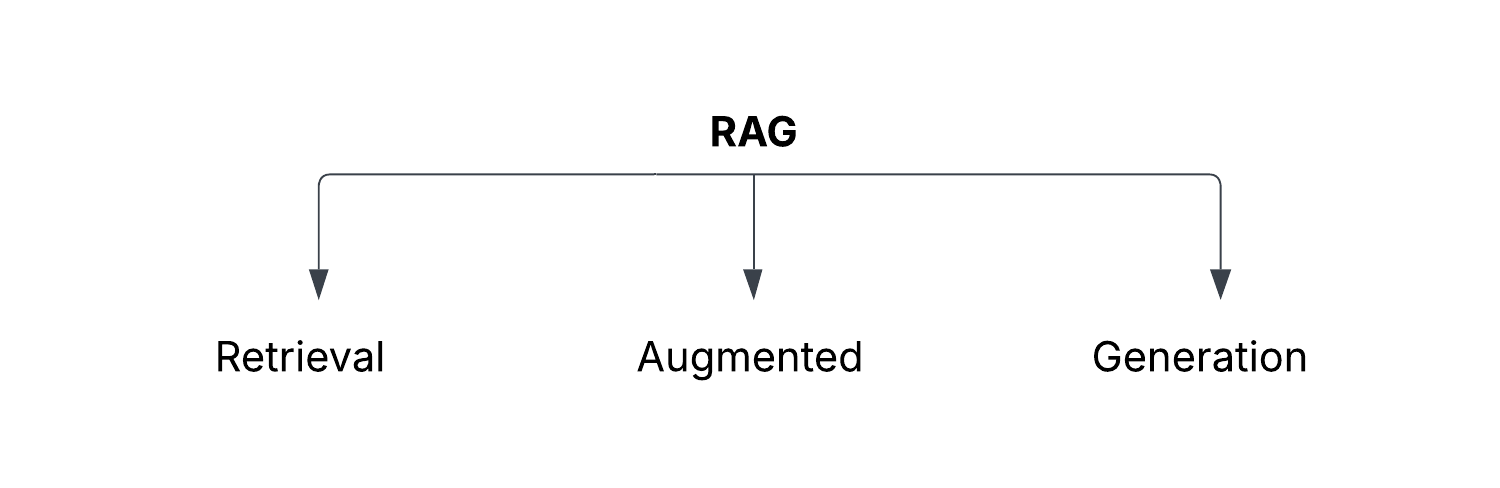
\includegraphics[width=0.8\linewidth]{figures/RAGDefinizione.png}
    \label{fig:significa-RAG}
\end{figure}
\section{Introduzione}
RAG \textbf{Retrieval-Augmented Generation}, (in italiano \textit{Generazione Aumentata tramite Recupero} )  è un sistema che permette di migliorare l'output di un LLM estendendo la sua conoscenza con nuove informazioni, al di fuori dai suoi dati di addestramento allo scopo di:
\begin{itemize}
    \item ottenere risposte mirate e personalizzate contenti knowledge relativa a librerie e codice custom;
    \item migliorare il codice generato rendendolo più specifico al dominio riducendo le allucinazioni;
    \item facilitare l'assistenza da parte del modello nella fase di debugging migliorando la sua comprensione di sistemi complessi;
    \item supportare la creazione di documentazione aggiornata;
    \item permettere all'interno di un Team di migliorare la coerenza del codice scritto da diversi programmatori proponendo librerie e standard comuni;
    \item evitare risposte imprecise a causa della confusione terminologica, in cui diverse fonti utilizzano la stessa terminologia per parlare di cose diverse.
\end{itemize}
\newpage
\section{Funzionamento}
Il sistema RAG si integra al LLM attivando un meccanismo di recupero delle informazioni per aumentare il prompt della richiesta.
Il funzionamento si articola in diverse fasi qui sotto illustrate:
\newline
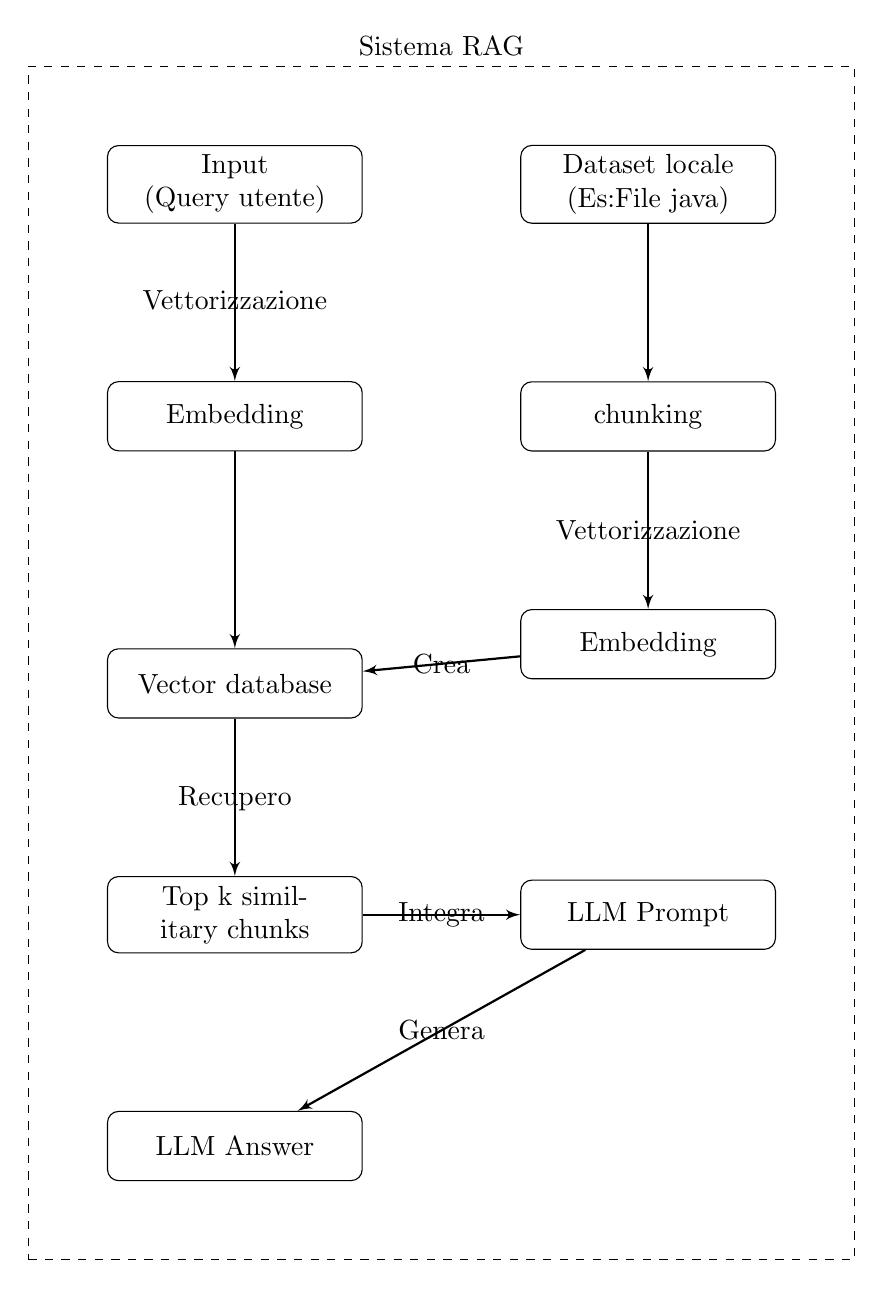
\begin{tikzpicture}[node distance=2cm]
    % Style definitions
    \tikzstyle{block} = [rectangle, draw, fill=white, 
        text width=3cm, text centered, rounded corners, minimum height=2.5em]
    \tikzstyle{line} = [draw, -latex', thick]
    \tikzstyle{data} = [text width=3cm, text centered]
    
    % Input nodes
    \node [block] (input) {Input\\(Query utente)};
    \node [block, right=of input] (docs) {Dataset locale\\(Es:File java)};
    
    % Processing nodes
  %  \node [block, below=of input] (query) {Query\\Processor};
    \node [block, below=of docs] (chunking) {chunking};
    
    % Embedding layer
    \node [block, below=of input] (qembed) {Embedding};
    \node [block, below=of chunking] (dembed) {Embedding};
    
    % Storage and retrieval
    \node [block, below=2.5cm of qembed] (vector) {Vector database};
    
    % LLM components
    \node [block, below=of vector] (context) {Top k similitary chunks};
    \node [block, right=of context] (llm) {LLM Prompt};
    \node [block, below=of context] (output) {LLM Answer};
    
    % Connections
    \path [line] (input) -- (qembed);
    \path [line] (docs) -- (chunking);
   % \path [line] (query) -- (qembed);
    \path [line] (chunking) -- (dembed);
    \path [line] (qembed) -- (vector);
    \path [line] (dembed) -- (vector);
    \path [line] (vector) -- (context);
    \path [line] (context) -- (llm);
    \path [line] (llm) -- (output);
    
    % Box around everything
    \node [draw, dashed, fit=(input) (docs) (chunking) (qembed) 
        (dembed) (vector) (context) (llm) (output),
        inner sep=1cm, label=above:Sistema RAG] {};
        
    % Add data flow labels
    \node [data] at ($(input)!0.5!(qembed)$) {Vettorizzazione};
    \node [data] at ($(chunking)!0.5!(dembed)$) {Vettorizzazione};
    \node [data] at ($(dembed)!0.5!(vector)$) {Crea};
    \node [data] at ($(vector)!0.5!(context)$) {Recupero};
    \node [data] at ($(context)!0.5!(llm)$) {Integra};
    \node [data] at ($(llm)!0.5!(output)$) {Genera};
\end{tikzpicture}

%\begin{figure}[h]
%    \centering
%    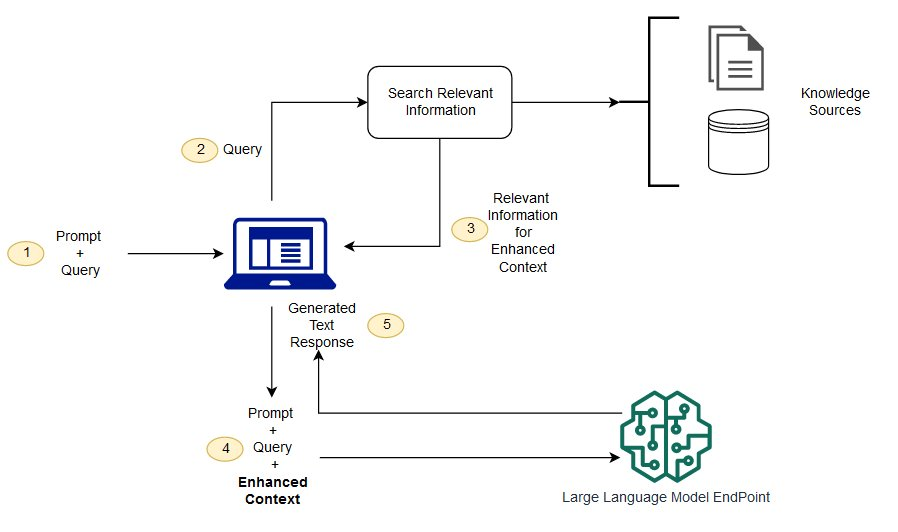
\includegraphics[width=.8\linewidth]{figures/jumpstart-fm-rag.jpg}
%    \caption{Flusso di una request ad un LLM integrato con un RAG}
%    \label{fig:jumpstart-fm-rag}
%\end{figure}

\subsection{Creazione Vector Database}
La propria \emph{knowledge base} deve essere salvata in un database vettoriale, in modo da poter essere interrogata in maniera efficiente dal sistema RAG.
Per creare questo database vengono utilizzati dati esterni al training set originale del LLM, provenienti da diverse fonti come:
\begin{itemize}
    \item API e database interni
    \item Archivi documentali
    \item File di testo e codice
\end{itemize}
La creazione di un database ben strutturato e la parte più importante di tutto il processo, dividere il codice in chunk correttamente etichettando ogni elemento con i corretti metadati è fondamentale per la sucessiva fase di interrogazione.
Il processo di creazione del Vector Database segue la seguente pipeline:
\begin{itemize}
    \item \textbf{Chunking}: Divisione del codice in chunk 
    \item \textbf{Embedding}: Conversione dei chunk in vettori numerici
    \item \textbf{Vector Store}: Memorizzazione degli embedding in un database vettoriale
\end{itemize}
%Creazione degli Embedding


\subsection{FASE 1: User query e function calling}
Data la query d'input da parte dell'utente, il sistema RAG è avviato da una chiamata di funzione per ricercare nel
\textbf{Vector Database} i chunk più rilevanti per la query.
Nei modelli più complessi in RAG è di fatto un agente integrato nel sistema che viene chiamato all'occorreza qunado la base di conoscenza del LLM non è sufficiente per fornire una risposta adeguata,
in questo modo viene anche razionalizzato e ottimizzato il costo computazionale del processo,
attivato solo quando strettamente neceassario.
Rimane comunque questo passaggio una scelta configurabile in base allo specifico utilizzo del sistema,
ad esempio per un azienda che utilizza il LLM solo per compiti specifici può essere configurato il sistema in modo che chiamii
la funzione RAG sempre.
\subsection{Fase 2: Recupero delle Informazioni}
Quando l'utente sottopone una query:
\begin{itemize}
    \item La domanda viene convertita in un vettore
    \item Il sistema cerca nel database vettoriale le informazioni più pertinenti
    \item Viene calcolata la rilevanza attraverso calcoli matematici vettoriali
\end{itemize}

\begin{figure}[h]
    \raggedright
    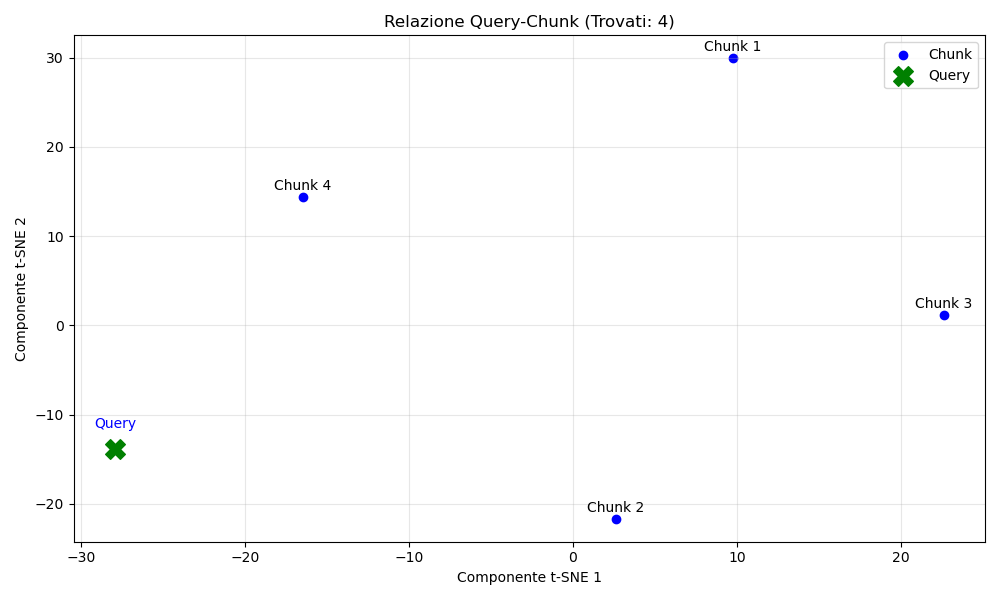
\includegraphics[width=0.8\linewidth]{figures/plotSearch.png}
    \label{fig:Emempio distanze chunk e query}
\end{figure}

\subsection{Fase 3: Aumento del Prompt}
Se trovate, il sistema RAG arricchisce il prompt dell'utente con le informazioni recuperate, fornendo al LLM un contesto più ampio e dettagliato per generare una risposta coerente.

\section{Perchè RAG}
Il RAG permette di superare le limitazioni di conoscenza dei LLM, fornendo risposte accurate e contestualizzate 
grazie all'integrazione di conoscenze interne e personalizzate.
Dopo aver costruito un sistema RAG è possibile eseguire rapidamente aggiornamenti al \textbf{Vector database},
cosa che sarebbe molto più difficile da ottenere con il fine-tuning, che richiede tempo e risorse significative.
Avere un LLM addestrato fin da subito su misura per le proprie sarebbe fantastico ma per quasi
tutte le aziende richiede risorse impossibili da sostenere ed è quindi molto più facile costruire un RAG
che intervenire direttamente sulla conoscenza del LLM solitamente di proprietà di terzi.

\chapter{Implementazione di un Sistema RAG per lo Sviluppo di codice per il linguaggio Java}
\section{Obiettivo}
Questo caso studio si propone di verificare il livello di personalizzazione e qualità delle risposte di un LLM potenziando la query nel prompt di input 
attraverso la creazione di un sistema RAG di supporto, analizzando singolarmente le varie fasi che compongono il processo.
Il sistema RAG è testato con della \textbf{classi JAVA uniche} create appositamente per il caso studio.
\subsubsection{Problematica da affrontare:}
Chiamate a più livelli di classi e metodi, dove il RAG potrebbe non essere in grado di estrapolare
le informazione necessarie da inserire nel prompt per ottenere dal LLM risposte coerenti con quanto richiesto.

\section{Architettura del Sistema}
\begin{figure}[h]
    \centering
    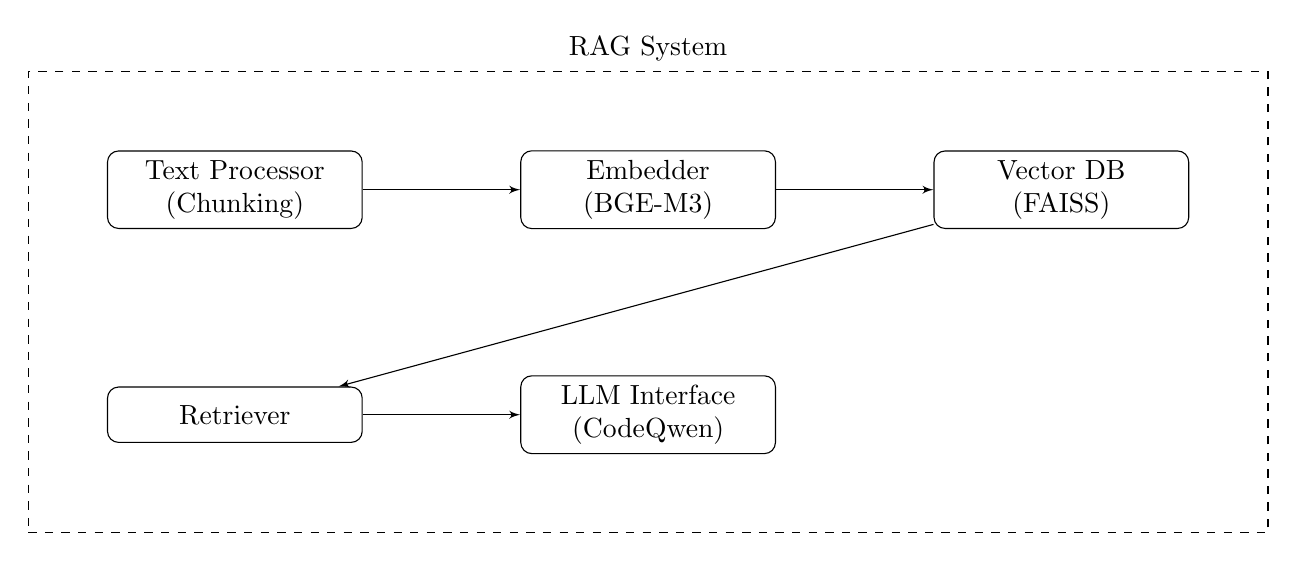
\begin{tikzpicture}[node distance=2cm]
        % Components
        \node [block] (chunk) {Text Processor\\(Chunking)};
        \node [block, right=of chunk] (embed) {Embedder\\(BGE-M3)};
        \node [block, right=of embed] (db) {Vector DB\\(FAISS)};
        \node [block, below=of chunk] (retriever) {Retriever};
        \node [block, right=of retriever] (llm) {LLM Interface\\(CodeQwen)};
        
        % Connections
        \path [line] (chunk) -- (embed);
        \path [line] (embed) -- (db);
        \path [line] (db) -- (retriever);
        \path [line] (retriever) -- (llm);
        
        % Box around everything
        \node [draw, dashed, fit=(chunk) (embed) (db) (retriever) (llm),
            inner sep=1cm, label=above:RAG System] {};
    \end{tikzpicture}
    \caption{Architettura del sistema RAG}
    \label{fig:rag-architecture}
\end{figure}
Il sistema RAG implementa un'architettura modulare composta da cinque componenti principali:

\begin{enumerate}
    \item \textbf{Text Processor (Chunking)}:
    \begin{itemize}
        \item Suddivide i file Java in chunk di un numero definito appositamente di token
        \item Gestisce sovrapposizione di token tra chunk
        \item Preserva il contesto del codice
    \end{itemize}

    \item \textbf{Embedder (BGE-M3)}:
    \begin{itemize}
        \item Converte i chunk in vettori numerici
        \item Utilizza il modello BGE-M3 per la generazione degli embedding
        \item Normalizza i vettori per ottimizzare la ricerca
    \end{itemize}

    \item \textbf{Vector DB (FAISS)}:
    \begin{itemize}
        \item Memorizza gli embedding in un database vettoriale
        \item Ottimizza la ricerca per similarità
        \item Garantisce recupero efficiente dei chunk rilevanti
    \end{itemize}

    \item \textbf{Retriever}:
    \begin{itemize}
        \item Esegue query semantiche sul database
        \item Recupera i k chunk più rilevanti
        \item Prepara il contesto per il LLM
    \end{itemize}

    \item \textbf{LLM Interface (CodeQwen e Llama 3.2)}:
    \begin{itemize}
        \item Interfaccia con i modelli CodeQwen e Llama 3.2
        \item Genera risposte basate sul contesto recuperato
        \item Ottimizza il prompt per la generazione di codice
    \end{itemize}
\end{enumerate}

\section{Software Utilizzati}
\subsection{Ollama\hspace{0.3cm}\protect
\includegraphics[width=0.03\linewidth]{figures/ollama.png}}
Ollama \cite{ollama-docs} è un software che permette di utilizzare in locale LLM
senza dover dipendere da servizi cloud esterni.
Il software è stato scelto per la sua flessibilità, permettendo di integrare facilmente i modelli LLM nel sistema RAG.
\subsection{LLM}
Ogni LLM è specializzato per determinati scopi,
per questo motivo per rendere più completa la ricerca sono stati utilizzati due modelli con caratteristiche differenti:
\subsubsection{Llama 3.2}
Llama 3.2 3B \cite{llama3-2}, un modello di linguaggio open source.
Il modello, con 3 miliardi di parametri, è ottimizzato per compiti di dialogo multilingue e si distingue per le sue capacità di recupero e sintesi delle informazioni.
La scelta è ricaduta su questa versione per il suo equilibrio tra prestazioni e requisiti computazionali che permottono il suo utilizzo senza hardware troppo potente.

\subsubsection{Codeqwen 1.5}
Codeqwen \cite{codeqwen1.5} è un modello di linguaggio open source specializzato nella generazione di codice e documentazione tecnica.  
Con 7 miliardi di parametri, il modello è stato addestrato su un ampio dataset di codice sorgente e documentazione tecnica, permettendo di generare codice coerente e ben strutturato.
La scelta di questo modello è stata dettata, a differenza di llama3.2, dalla sua specializzazione nella programmazione e dalla sua capacità di generare codice di alta qualità. 
%\subsubsection{qwen2.5-coder:3b}
%qwen2.5-coder \cite{qwen-coder} è stato sviluppato da Qwen AI ed è anchesso open source, specializzato nella generazione di codice e documentazione tecnica.
%Con 3 miliardi di parametri, il modello è stato addestrato su un ampio dataset di codice sorgente e documentazione tecnica, permettendo di generare codice coerente e ben strutturato. 
%La scelta di questo modello è stata dettata, a differenza di llama3.2, dalla sua specializzazione nella programmazione e dalla sua capacità di generare codice di alta qualità.

\subsection{LangChain}
LangChain \cite{langchain} è un framework open source progettato per costruire applicazioni basate su LLM.
Fornisce strumenti avanzati per integrare modelli con dati esterni ed API, creare pipeline con chain
e gestire database vettoriali, supportando l'implementazione di sistemi RAG.

\subsection{BGE-M3}
BGE-M3 \cite{bge-m3} è un modello di embedding testuale open source per la gestione di dati strutturati e non strutturati multilingue.
Il modello permettendo di convertire testo in vettori numerici ad alta dimensionalità.

\subsection{FAISS}
FAISS (Facebook AI Similarity Search) \cite{faiss} è una libreria open source per la ricerca efficiente di similarità e il clustering di vettori densi.
Progettata per gestire dataset su larga scala, FAISS supporta operazioni di ricerca anche su insiemi di vettori che superano la capacità della RAM, grazie a tecniche di indicizzazione avanzate e ottimizzazioni computazionali.

\section{Dataset}
Il dataset creato appositamente è composto da tre classi Java:

\begin{description}
    \item[DateUtilCustom.java] Classe personalizzata per gestire le date
    \item[GiorniMagici.java] Classe per calcolare in maniera particolare dei giorni
    \item[BasketballStats.java] Classe per calcolare statistiche relative al mondo del basket.
\end{description}

\section{Scenario base del Caso Studio}
La classe BasketballStats.java non ha nessuna relazione con le altre due classi,
mentre DateUtilCustom.java e GiorniMagici.java sono strettamente correlate infatti GiorniMagici.java richiama metodi presenti in DateUtilCustom.java.
Andremo a testare il sistema RAG con la seguente query: 
\begin{itemize}
    \item \textbf{Cosa ritorna il metodo \texttt{segnaleWow(LocalDate.of(2025, 2, 14))}?}
\end{itemize}

\subsection{Codice di riferimento per rispondere alla query}
In GiorniMagici.java è presente la seguente funzione:
\begin{lstlisting}[language=Java, caption={Metodo segnaleWow in GiorniMagici.java}, label={lst:segnaleWow}]
public static String segnaleWow(LocalDate data) {
    String wow = "il tuo segnale Wow e': " + DateUtilCustom.getMessaggioMagico(date);
    return wow;
}
\end{lstlisting}
Questa funzione richiama il metodo \texttt{getMessaggioMagico} presente in DateUtilCustom.java:

\begin{lstlisting}[language=Java, caption={Metodo getMessaggioMagico in DateUtilCustom.java}, label={lst:getMessaggioMagico}]
public static String getMessaggioMagico(LocalDate datamagica) throws DateTimeParseException {
    DayOfWeek giornoSettimana = datamagica.getDayOfWeek();
    switch(giornoSettimana) {
        case MONDAY: return "La magia inizia nel silenzio...";
        case TUESDAY: return "I sussurri degli antichi si fanno sentire.";
        case WEDNESDAY: return "Il velo tra i mondi e' sottile oggi.";
        case THURSDAY: return "L'energia magica e' potente e chiara.";
        case FRIDAY: return "Attenzione agli incantesimi del crepuscolo.";
        case SATURDAY: return "Il giorno perfetto per scoprire segreti nascosti.";
        case SUNDAY: return "Riposa e rigenera il tuo potere magico.";
        default: return "Il giorno e' avvolto nel mistero...";
    }
}
\end{lstlisting}

\subsection{Risultato Atteso}
Essendo il 14 Febbraio 2025 un venerdì, ci aspettiamo come risposta:
\begin{quote}
    \textbf{``il tuo segnale Wow è: Attenzione agli incantesimi del crepuscolo.''}
\end{quote}

\section{Implementazione}
\subsection{Creazione dei Chunk}
I modelli di embedding hanno limiti massimi di input (512-4096 token)  per questo spezzare il codice in chunk di dimensioni adeguate è obbligatorio oltre ad essere in ogni caso fondamentale.
Inoltre occorre prestare attenzione alla dimensione dei chunk generati, se troppo piccoli riducono il contesto disponibile per il modello mentre se troppo grandi perdono focalizzazione semantica.
Per suddividere il file Java in chunk viene utilizzata la libreria \textbf{langchain\_text\_splitters.}
Il seguente codice Python mostra come suddividere i file Java in chunk di dimensione fissa, salvando i risultati in un file JSON.
\begin{lstlisting}[language=Python, caption={Codice Python per la suddivisione dei file Java in chunk}, label={lst:chunking}]
    from langchain_text_splitters import RecursiveCharacterTextSplitter
    import json
    
    # Funzione per caricare e suddividere un file Java
    def process_file(file_path):
        with open(file_path, "r", encoding="utf-8") as f:
         lines = f.readlines()
    
        # Ricostruisce il testo mantenendo le informazioni sulle linee
        text = ''.join(lines)
    
        splitter = RecursiveCharacterTextSplitter(
        chunk_size=256, #molto basso per prevenire merge di metodi
        chunk_overlap=64,
        separators=[
            # I seguenti separatori sono stati usati per mantenere i metodi uniti
            # Prioritari: catturano la fine dei metodi
            "\n}\n\npublic ",
            "\n}\n\nprivate ",
            "\n}\n\nprotected ",
            "\n}\n\nstatic ",
            "\n}\n\n// End of method", 
            
            # Secondari: separatori generici
            "\n}\n",  # Qualsiasi chiusura di blocco
            "\nclass ",  # Inizio nuove classi
            "\n@",  # Annotazioni
            "\n/**",  # Javadoc
            "\n * ", 
            "\n"
        ],
        keep_separator=False, # per evitare riporto di separatori
        is_separator_regex=False
    )
    
        chunks = splitter.split_text(text)
        # Calcola le linee esatte per ogni chunk
        chunk_metadata = []
        cursor = 0
        for chunk in chunks:
            start_line = text.count('\n', 0, cursor) + 1
            chunk_length = len(chunk)
            end_line = text.count('\n', 0, cursor + chunk_length) + 1
            chunk_metadata.append({
                "start_line": start_line,
                "end_line": end_line,
                "text": chunk
            })
            cursor += chunk_length
        
        return chunk_metadata
    
    # Carica e suddividi i file Java
    files = ["my_project/DateUtilCustom.java", "my_project/GiorniMagici.java", "my_project/BasketballStats.java"]
    all_chunks = []
    
    for file_path in files:
        chunks_info = process_file(file_path)
        for chunk_info in chunks_info:
            chunk_text = chunk_info["text"]
            
            # Aggiungi contesto strutturale
            class_context = ""
            if "class " in chunk_text:
                class_name = chunk_text.split("class ")[1].split("{")[0].strip()
                class_context = f"Classe: {class_name}\n"
            
            all_chunks.append({
                "id": len(all_chunks) + 1,
                "text": f"// File: {file_path}\n{class_context}{chunk_text}",
                "source": file_path,
                "type": "code",
                "start_line": chunk_info["start_line"],
                "end_line": chunk_info["end_line"],
                "class": class_context.replace("Classe: ", "") if class_context else ""
            })
    
    # Salva i chunk in un file JSON
    with open("chunks.json", "w", encoding="utf-8") as f:
        json.dump(all_chunks, f, indent=4, ensure_ascii=False)
\end{lstlisting}
Il chunking è costruito in maniera specifica per \textbf{codice java}, i separatori sono stati scelti per tentare di segmentare il codice secondo la struttura tipica dei metodi e delle classi, garantendo che il chunk contenga blocchi di codice "interi".
L'opzione \texttt{keep\_separator=False} crea punti di split più naturali per il codice Java, allineandosi meglio con la struttura dei metodi e delle classi.
Per ciascun chunk, se nel testo è presente la stringa \texttt{class}, il codice estrae il nome della classe 
(prendendo il testo che segue \texttt{class} fino al primo \texttt{\{}) e lo utilizza per creare un contesto 
strutturale (es \texttt{Classe: NomeClasse}).
Questo contesto viene preappeso al testo del chunk e salvato anche come valore nel campo "class".

\subsubsection{Il risultato nel file chunks.json è il seguente:}
    \begin{lstlisting}[language=json,firstnumber=1, caption={Esempio di chunks generati}, label={lst:chunks-example}]
        [
            {
                "id": 1,
                "text": "// File: my_project/DateUtilCustom.java\nimport java.text.ParseException;\nimport java.text.SimpleDateFormat;\nimport java.time.DayOfWeek;\nimport java.time.LocalDate;\nimport java.time.format.DateTimeParseException;\nimport java.util.Calendar;\nimport java.util.Date;",
                "source": "my_project/DateUtilCustom.java",
                "type": "code",
                "start_line": 1,
                "end_line": 7,
                "class": ""
            },
            {
                "id": 2,
                "text": "// File: my_project/DateUtilCustom.java\nClasse: DateUtilCustom\nimport java.util.Calendar;\nimport java.util.Date;\nimport java.util.concurrent.TimeUnit;\npublic class DateUtilCustom {\n    /**\n     * Formatta una data nel formato \"dd/MM/yyyy\".\n     *\n     * @param date La data da formattare.",
                "source": "my_project/DateUtilCustom.java",
                "type": "code",
                "start_line": 7,
                "end_line": 16,
                "class": "DateUtilCustom\n"
            }
            ............continua
        ]
    \end{lstlisting}
        
    Ogni chunk mantiene:
    \begin{itemize}
        \item Il riferimento al file sorgente
        \item Il nome della classe
        \item Le righe di inizio e fine nel file originale
        \item Il contenuto del codice con la sua struttura
    \end{itemize}

\subsection{Arricchire i chunk con metadati relativi al codice}
    Oltre al testo del codice, è importante mantenere informazioni aggiuntive per facilitare la ricerca e l'interpretazione dei chunk.
    La seguente funzione \texttt{extract\_method\_name} aggiunge una stringa contestuale per ogni chunk che include:
    \begin{itemize}
        \item Il nome del metodo o della classe
        \item La classe di appartenenza
        \item Le righe di inizio e fine del codice
    \end{itemize}

    \begin{lstlisting}[language=Python, caption={Funzione extract\_method\_name}]
    import re
    def extract_method_name(text):
        # Pattern per la firma di un metodo in Java
        method_pattern = r'(?:public|private|protected|static|final|synchronized|abstract|native)\s+[\w<>\[\]]+\s+(\w+)\s*\([^)]*\)'
        
        # Pattern per i costruttori
        constructor_pattern = r'(?:public|private|protected)\s+(\w+)\s*\([^)]*\)'
        
        # Cerca la firma di un metodo
        matches = re.findall(method_pattern, text)
        if matches:
            return matches[0]  # Restituisce il primo metodo trovato
        
        # Cerca costruttori
        constr_matches = re.findall(constructor_pattern, text)
        if constr_matches:
            return constr_matches[0] + " (costruttore)"
        
        # Cerca chiamate a metodi
        method_calls = re.findall(r'\.(\w+)\s*\(', text)
        if method_calls:
            return f"Chiamata a: {method_calls[-1]}"
        
        return "unknown_method"  # Default se non trova nulla
    \end{lstlisting}
        
\subsection{Generazione degli Embedding}
    Gli embedding trasformano i chunk in rappresentazioni vettoriali che catturano il significato semantico.
    Il seguente codice Python mostra come generare gli embedding e creare un database Faiss.
    Come precedentemente descritto, il modello di embedding utilizzato è BGE-M3, questo modello usa due rappresentazioni per complementarietà, la rappresentazione denza cattura relazioni semantiche mentre quella sparsa cattura relazioni sintattiche.
    Mentre sul database FAISS ad alta dimensionalità verrà settata la ricerca di somiglianza utilizzando la distanza euclidea tra i vettori.
    
    \begin{lstlisting}[language=Python, caption={Codice Python per la generazione degli embedding e la creazione di un database FAISS}, label={lst:embeddings}]
        import json
        from sentence_transformers import SentenceTransformer
        from langchain_community.vectorstores import FAISS
        
        # 1. Carica i chunk dal file JSON
        with open("chunks.json", "r", encoding="utf-8") as f:
            chunks_data = json.load(f)
        
        chunks = [item["text"] for item in chunks_data]
        
        # 2. Carica il modello BGE-M3 e genera gli embedding
        embedder = SentenceTransformer('BAAI/bge-m3')
        embeddings = embedder.encode(
            [f"METHOD:{extract_method_name(c['text'])} CLASS:{c['class']} LINES:{c['start_line']}-{c['end_line']} CONTENT:{c['text']}" 
             for c in chunks_data],
            show_progress_bar=True
        )
        
        # 3. Crea un database FAISS
        vector_store = FAISS.from_embeddings(
            text_embeddings=list(zip(chunks, embeddings)),  # Abbina testi e embedding
            embedding=embedder,  # Modello per future operazioni
        )
        
        # 4. Salva il database
        vector_store.save_local("./faiss_db")
        print("Database FAISS creato e salvato in ./faiss_db.")
    \end{lstlisting}

Il metodo \emph{encode()} del modello BGE-M3 genera gli embedding per ogni chunk,
chiamando la funzione \emph{extract\_method\_name} per arricchire il contesto e creare vettori con relazioni semantiche strutturate.

\subsection{Esecuzione di query sul Database FAISS}
    Una volta creato il database FAISS, è possibile eseguire ricerche semantiche sui chunk memorizzati:

    \begin{lstlisting}[language=Python, caption={Esecuzione di una query sul database FAISS}, label={lst:query}]
    from langchain_community.vectorstores import FAISS
    from langchain_huggingface import HuggingFaceEmbeddings

    # 1. Carica il modello di embedding nel formato corretto
    embedder = HuggingFaceEmbeddings(
        model_name="BAAI/bge-m3",
        model_kwargs={'device': 'cpu'},
        encode_kwargs={'normalize_embeddings': True}
    )

    # 2. Carica il database FAISS esistente
    vector_store = FAISS.load_local(
        folder_path="./faiss_db",
        embeddings=embedder,
        allow_dangerous_deserialization=True
    )

    # 3. Query di esempio
    query = "Cosa ritorna il metodo segnaleWow(LocalDate.of(2025, 1, 10))?"

    # 4. Cerca i chunk piu' simili
    docs = vector_store.similarity_search_with_score(
        query,
        k=5,
        score_threshold=0.90,  # bassa similarita'
        search_type="similarity",  # Piu' efficace per il codice
        lambda_mult=0.5       # Bilancia diversita'/rilevanza
    )

    # 5. Stampa i risultati con relativo score
    for i, (doc, score) in enumerate(docs):
        print(f"Risultato {i+1} (Score: {score:.4f}):")
        print(doc.page_content)
        print("-" * 40)
    \end{lstlisting}

    \subsubsection{Risultati con query base (senza alcun riferimento al metodo utilizzato all'interno di segnale Wow)}
    \begin{itemize}
        \item \textbf{Query:} 
            \newline
                \textbf{``Cosa ritorna il metodo segnaleWow(LocalDate.of(2025, 1, 10))?''}
            \newline
        \item \textbf{Output:}
        viene restituito il chunk corretto con uno score di similarità di \textbf{0.6547}. Questo valore, basato sulla cosine similarity, non è particolarmente alto ma sufficiente per identificare il chunk corretto.
    \end{itemize}
    \paragraph{Nota:}
    È importante riscontrare che viene restituito un solo chunk nonostante \texttt{k=5}.
    Questo accade perché nessun altro chunk supera la soglia di similarità impostata.
    Tale comportamento evidenzia una criticità: la funzione \texttt{segnaleWow} richiama un metodo presente nella libreria \texttt{DateUtilCustom} che non viene estratto dal Dataset.

    \subsubsection{Riformulazione query (aggiungendo riferimento al metodo utilizzato all'interno di segnale Wow)}
        \begin{itemize}
            \item \textbf{Per risolvere questo problema, la query è stata riformulata:}
            \begin{quote}
                \textbf{``Cosa ritorna il metodo segnaleWow(LocalDate.of(2025, 1, 10)) che utilizza la funzione getMessaggioMagico() della libreria DateUtilCustom?''}
            \end{quote}
            \item \textbf{L'output fornisce 5 risultati:}
            \begin{itemize}
                \item Primo chunk \textbf{(score: 0.5276)}: contiene la funzione \texttt{segnaleWow}
                \item Secondo, terzo e quarto chunk \textbf{(scores: 0.7188, 0.7258, 0.7605)}: contengono la funzione \texttt{getMessaggioMagico}
                \item Quinto chunk \textbf{(score: 0.8958)}: funzione non rilevante relativa alle date
            \end{itemize}
        \end{itemize}

    \paragraph{Conclusione:}
    Sono state riscontrate due problematiche molto rilevanti, la prima riguarda la mancanza di estrazione di metodi da librerie esterne se non esplicitate nella query.
    Mentre la seconda guarda i chunck estratti, lo score ottenuto non è particolarmente alto e questo con un database più ampio potrebbe portare a risultati non coerenti.
    Per il secondo punto questa analisi ha portato alla decisione di abbassare \texttt{score\_threshold} da 0.90 a 0.80,
    questa piccola correzione risolve in parte la problematica o almeno evita di propagarla ulteriormente preferendo non ottenere risultati piuttosto che ricevere risposte non coerenti.
    
\subsection{Creazione della Pipeline RAG}
\begin{lstlisting}[language=Python, caption={Pipeline RAG}, label={lst:rag}]
    from langchain_community.vectorstores import FAISS
    from langchain_huggingface import HuggingFaceEmbeddings
    from langchain_ollama import OllamaLLM
    from langchain.chains import create_retrieval_chain
    from langchain.chains.combine_documents import create_stuff_documents_chain
    from langchain.prompts import PromptTemplate
    
    # Configurazione embedding
    embedder = HuggingFaceEmbeddings(
        model_name="BAAI/bge-m3",
        model_kwargs={'device': 'cpu'},
        encode_kwargs={'normalize_embeddings': True}
    )
    
    # Caricamento database FAISS
    vector_store = FAISS.load_local(
        folder_path="./faiss_db",
        embeddings=embedder,
        allow_dangerous_deserialization=True
    )
    # Aggiunta del database FAISS al retriever
    retriever=vector_store.as_retriever(
            search_kwargs={
                "k": 5,                   # Piu' documenti per contesto
                "score_threshold": 0.80, # medio-bassa similarita' inizialmente era 0.90
                "search_type" :"similarity",  # Piu' efficace per il codice
                "lambda_mult":0.5       # Bilancia diversita'/rilevanza
            }
        )
    
    varStileLLM = "Sei un programmatore che risponde conciso ma sintetico."
    
    # Configurazione Template del prompt specifici per i modelli
    LLAMA_TEMPLATE = """<|begin_of_text|>
    <|start_header_id|>system""" + varStileLLM + """<|end_header_id|>
    Contesto: {context}<|eot_id|>
    <|start_header_id|>user<|end_header_id|>
    Domanda: {input}<|eot_id|>
    <|start_header_id|>assistant<|end_header_id|>"""
    
    CODEQWEN_TEMPLATE = """<|im_start|>system """ + varStileLLM + """
    {context}<|im_end|>
    {{ if .Functions }}<|im_start|>functions
    {{ .Functions }}<|im_end|>{{ end }}
    <|im_start|>user
    {input}<|im_end|>
    <|im_start|>assistant
    """
    
    COMMON_PARAMS = {
        "temperature": 0.3, #lasciamo una bassa creativita' non vogliamo che inventi risposte
        "top_p": 0.85  # Bilancia creativita'/controllo nei token generati
    }
    
    # Caricamento modello
    def load_model(model_name):
        models = {
            "llama3.2": {
                "template": LLAMA_TEMPLATE,
                "params": COMMON_PARAMS
            },
            "codeqwen": {
                "template": CODEQWEN_TEMPLATE,
                "params": COMMON_PARAMS
            }
        }
        if model_name not in models:
            raise ValueError(f"Modello non supportato: {model_name}")
        return OllamaLLM(
            model=model_name,
            **models[model_name]["params"]
        ), PromptTemplate(
            template=models[model_name]["template"],
            input_variables=["input", "context"]
        )
    
    # Inizializza il modello
    llm, prompt = load_model("codeqwen")
    
    # Catena RAG
    document_chain = create_stuff_documents_chain(llm, prompt)
    rag_chain = create_retrieval_chain(
        retriever,
        document_chain
    )
    
    # Funzione query
    def ask_ollama(question):
        try:
            result = rag_chain.invoke({"input": question})
            print("DOMANDA:", question)
            print("RISPOSTA:")
            print(result["answer"])
            print("FONTI:")
            for i, doc in enumerate(result["context"], 1):
                print(f"{i}. {doc.page_content[:150]}...")
                if 'source' in doc.metadata:
                    print(f" Fonte: {doc.metadata['source']}")
                print("-" * 80)
        except Exception as e:
            print(f"ERRORE: {str(e)}")
    
    # Esempio d'uso
    if __name__ == "__main__":
        ask_ollama("Cosa ritorna il metodo segnaleWow(LocalDate.of(2025, 1, 10)) che utilizza la funzione getMessaggioMagico() della libreria DateUtilCustom?")
        #ask_ollama("Cosa ritorna il metodo segnaleWow(LocalDate.of(2025, 1, 10))?")
\end{lstlisting}
\subsubsection{Spiegazione Pipeline del RAG}
    Seguendo la struttura precedentemente creata, per eseguire l'embedder della query di input viene utilizzato il modello BAAI/bge-m3 e
    caricato il database FAISS contenente la \textbf{knowledge base}.
    La chiamata iniziale alla funzione \emph{ask\_ollama()} richiede come parametro \textbf{la query di input} che verrà processata dalla pipeline RAG.
    Sfruttando le funzionalità della libreria LangChain \cite{langchain-retrieval-chain}, \textbf{\emph{result}} sarà un array contente la risposta("answer") e il contesto("context") fornito alla query.
\subsubsection{\emph{rag\_chain.invoke()}}
 Questa funzione esegue la catena RAG creata tramite il metodo \emph{create\_retrieval\_chain()} che prende come parametri il retriever e il document chain.
 \begin{itemize}
    \item la funzione \textbf{create\_stuff\_documents\_chain()} carica una catena di documenti prendendo in input il modello LLM e il template del prompt.
    \item \textbf{load\_model()} carica il modello LLM e il template del prompt in base al modello scelto sfruttando OllamaLLM e PromptTemplate.
 \end{itemize}
 \subsubsection{Temperature}
Per i due LLM è stata data una temperature molto bassa \textbf{0.3} in modo da garantire da parte dei LLM risposte coerenti e precise senza provi ad inventarle.
\subsubsection{Top\_p}
Il parametro \texttt{top\_p} è stato impostato a 0.85 per bilanciare creatività e controllo nei token generati.
\subsubsection{System}
Come parametro di sistema da passare al LLM è stato esplicitamente richiesto di rispondere in italiano come esperto di programmazione ma solo se è sicuro.

\section{Test Sistema RAG}
Valutiamo se il sistema RAG  è in grado di rispondere in maniera coerente alla query proposta.
Ricordiamo che il risultato atteso è: \textbf{``il tuo segnale Wow è: Attenzione agli incantesimi del crepuscolo.''}    
\subsection{Query base senza riferimenti al metodo utilizzato all'interno di segnaleWow}
\begin{quote}
    \texttt{``Cosa ritorna il metodo segnaleWow(LocalDate.of(2025, 2, 14))?''}
\end{quote}
\subsubsection{Fonti aggiunte al prompt}
Il RAG aggiunge solo il chunk dove è presente la funzione \texttt{segnaleWow} e non il chunk con la funzione \texttt{getMessaggioMagico} della libreria DateUtilCustom
per questo le risposte dei due modelli sono incomplete:
\subsubsection{Output con LLM Llama3.2}
L'output ottenuto utilizzando il modello Llama3.2 è stato:
\begin{quote}
    ``Il metodo \texttt{segnaleWow} restituisce una stringa che contiene un messaggio magico associato alla data specificata. In questo caso, la data è il 14 Febbraio 2025.
La risposta esatta sarebbe:
"il tuo segnale Wow è : [messaggio magico]"
dove [messaggio magico] è il risultato dell'applicazione di `DateUtilCustom.getMessaggioMagico(date).''
\end{quote}

\subsubsection{Modifica Temperature}
CodeQwen provava a dare risposta anche senza avere tutte le informazioni necessarie, ho deciso di abbassare la temperatura da 0.3 a 0.2 per vedere se il modello CodeQwen avrebbe risposto in maniera più precisa.
Cosa che è avvenuta:

\subsubsection{Output con LLM CodeQwen}
Utilizzando invece il modello CodeQwen, la risposta ottenuta è stata:
\begin{quote}
    ``Se si chiama il metodo `segnaleWow` con un'istanza di `LocalDate` che rappresenta la data "14 febbraio 2025", il valore restituito sarà una stringa che indica il segnale Wow associato a tale data.
    ```java
    String result = GiorniMagici.segnaleWow(LocalDate.of(2025, 2, 14));
    System.out.println(result);
    ```
    Il metodo `getMessaggioMagico` viene richiamato su un'istanza di `DateUtilCustom`, passando la data "14 febbraio 2025" come parametro. Questo metodo presumibilmente restituisce un messaggio magico associato a tale data, ad esempio "La data del New Year è una data speciale".
    Il risultato finale sarà:
    ```
    il tuo segnale Wow è : La data del New Year è una data speciale``
\end{quote}

\subsection{Query Completa con riferimenti al metodo utilizzato all'interno di segnaleWow}
\begin{quote}
    \texttt{``Cosa ritorna il metodo segnaleWow(LocalDate.of(2025, 2, 14)) che utilizza la funzione getMessaggioMagico() della libreria DateUtilCustom?''}
\end{quote}
\subsubsection{Fonti aggiunte dal RAG al prompt}
In questo caso il RAG aggiunge 5 chunk, ovvero oltre a quello relativo alla funzione \texttt{segnaleWow} anche i chunk relativi alla funzione \texttt{getMessaggioMagico} della libreria DateUtilCustom.
Ne consegue che \textbf{le risposte date dai due modelli sono coerenti con quanto atteso}.
\subsubsection{Output con LLM Llama3.2}
``Il metodo `segnaleWow` restituisce una stringa che contiene il messaggio magico per la data specificata. 
Per determinare il messaggio esatto, dobbiamo analizzare la data fornita: `LocalDate.of(2025, 2, 14)`.
La data è il 14 febbraio 2025. Il giorno della settimana corrisponde a `FRIDAY`.
Quindi, il messaggio magico restituito dal metodo `getMessaggioMagico` sarà:
\textbf{"Attenzione agli incantesimi del crepuscolo."}''
\subsubsection{Output con LLM CodeQwen}
``Se si chiama il metodo `segnaleWow` con una data di `LocalDate.of(2025, 2, 14)`, utilizzando la funzione `getMessaggioMagico()` della libreria `DateUtilCustom`, il risultato sarà:
```
Il tuo segnale Wow è : \textbf{Il giorno perfetto per scoprire segreti nascosti.}
```
Questo è dato che la data 2025-02-14 cade mercoledì, quindi il metodo `getMessaggioMagico()` restituisce il messaggio "Il giorno perfetto per scoprire segreti nascosti.''
\subsection{Commento risultati ottenuti}
I risultati ottenuti mostrano come il sistema RAG sia in grado di rispondere in maniera coerente alla query proposta.
La ricerca dei chunk più simili funziona corrette soprattutto se si scrive la richiesta in maniera più dettagliata possibile.
CodeQwen ha sbagliato a calcolare il giorno della settimana ma la risposta utilizza correttamente il metodo getMessaggioMagico().

\section{Valutazione del RAG con llm as a judge}
Utilizzando l'approccio \textbf{\emph{"llm as a judge"}} per valutare automaticamente quanto prodotto dal sistema RAG
generiamo una serie di domande al sistema RAG operando una valutazione automatizzata delle risposte prodotte da parte di più LLM.
Il dataset è stato arricchito di altre classi java generate sinteticamente dal LLM Deepssek.
\subsection{Domande}
Passando il file contenente tutte le librerie a Deepseek, sono state generate 30 domande per valutare il sistema RAG.
La domanda fatta al LLM è stata:
\begin{quote}
    \texttt{``Dalle mie classi genera 30 domande/risposte per valutare il mio rag:
    la prima è: Cosa ritorna il metodo segnaleWow(LocalDate.of(2025, 2, 14))
    che utilizza la funzione getMessaggioMagico() della libreria
    DateUtilCustom?''}
\end{quote}
Il risulta è stato il seguente:
\begin{lstlisting}[language=Python, caption={Domande generate da Deepssek}]
    id,question,context
Q1,"Cosa ritorna il metodo segnaleWow(LocalDate.of(2025, 2, 14)) che utilizza la funzione getMessaggioMagico()?","GiorniMagici.java"
Q2,"Come calcolare la media battuta con 25 valide su 80 turni?","CalcolatoreStatisticheBaseball.java"
Q3,"Quale ERA risulta da 5 punti subiti in 7 inning?","CalcolatoreStatisticheBaseball.java"
Q4,"Come validare una password 'Secret123!'?","GestionePassword.java"
Q5,"Cosa restituisce invertiStringaMantenendoMaiuscole('AbCde')?","AnalizzatoreTesto.java"
Q6,"Come convertire 10km in miglia?","ConvertitoreUnita.java"
Q7,"Quale BMI risulta da 70kg e 1.75m?","CalcolatoreBMI.java"
Q8,"Cosa significa un momentum [12,15] vs [8,10]?","BasketballStats.java"
Q9,"Come cifrare 'HELLO' con Caesar shift 3?","StrumentiCrittografia.java"
Q10,"Quale temperatura a Roma (41.9) a luglio?","SimulatoreMeteo.java"
Q11,"Cosa restituisce isDataMagica(6, 5, 2030)?","GiorniMagici.java"
Q12,"Come calcolare rata mutuo 100k al 4\% in 20 anni?","GestioneFinanzePersonali.java"
Q13,"Cosa restituisce getMessaggioMagico(LocalDate.of(2024,12,25))?","DateUtilCustom.java"
Q14,"Come calcolare VAN al 5% per flussi [100,200,300]?","AnalizzatoreInvestimenti.java"
Q15,"Quale complessita' ciclomatica per codice con 3 if e 2 while?","AnalizzatoreCodice.java"
Q16,"Cosa restituisce modelloPredaPredatore(100,50,0.1,0.05)?","SimulatoreEcologico.java"
Q17,"Come generare password sicura di 12 caratteri?","GestionePassword.java"
Q18,"Cosa restituisce convertiGrigio(0xFFAABB)?","StrumentiGrafica.java"
Q19,"Come calcolare log base 3 di 27?","CalcolatriceScientifica.java"
Q20,"Quale categoria BMI per 28.7?","CalcolatoreBMI.java"
Q21,"Cosa restituisce isPastDate(1/1/2020)?","DateUtilCustom.java"
Q22,"Come aggiungere 15 giorni al 1/1/2024?","DateUtilCustom.java"
Q23,"Quale ROI per guadagno 1500 su costo 1000?","AnalizzatoreInvestimenti.java"
Q24,"Cosa restituisce calcolaEfficienzaGiocatore(20,10,8,2,5)?","BasketballStats.java"
Q25,"Come simulare crescita popolazione 1000 al 2% in 5 anni?","SimulatoreEcologico.java"
Q26,"Cosa restituisce analisiStatisticheSquadra(85, 70, 12, 28)?","BasketballStats.java"
Q27,"Come decifrare 'KHOOR' con Caesar shift 3?","StrumentiCrittografia.java"
Q28,"Quale percussocritico per attivita' [5,8,3]?","GestoreProgetti.java"
Q29,"Cosa restituisce giorniAlmiocompleannoSpecial(1/1/2000, 'Mario')?","DateUtilCustom.java"
Q30,"Come calcolare radice 5a di 3125?","CalcolatriceScientifica.java"
\end{lstlisting}
\subsection{Punteggio delle domande}
Per valutare le domande generate da \textbf{Deepssek}, è stato chiesto a \textbf{GPT4o} e a \textbf{Mistral} di 
fornire un "punteggio totale" che indichi la capacità di rispondere alla domanda senza ambiguità con il contesto dato.
Date la vostra risposta su una scala da 1 a 5, dove 1 significa che la domanda non è affatto risolvibile in base al contesto e 5 significa che la domanda è chiaramente e inequivocabilmente risolvibile in base al contesto.
\subsubsection{Risultati}
Entrambi i modelli hanno valutato le domande generate da Deepssek con un punteggio medio di 4.63 su 5:
\begin{itemize}
    \item \textbf{GPT4o}: 139 su 150
    \item \textbf{Mistral}: 139 su 150
\end{itemize}
\subsection{Risposta alle domande da parte dei LLM con RAG}
Essendo poco performanti le versioni dei LLM installati in locale, per questo test ho valutato di utilizzare le versioni commerciali di Deepseek, o1 in Copilot e Mistral 
presenti in rete per rispondere alle domande.
Fornendo per ogni domanda lo stesso prompt creato dal mio sistema RAG, arricchito con i chunk estratti dalla funzione vector\_store.similarity\_search\_with\_score precedentemente creata.
\subsection{Risultati}
miao
\chapter{Conclusioni}

da completare
%In questa tesi ho esplorato l'integrazione di RAG e LLM nello sviluppo del software, dimostrando come questi strumenti possano migliorare significativamente il processo di sviluppo. I risultati principali includono:
%\begin{itemize}
%    \item Implementazione di un sistema RAG per la generazione di codice contestualizzato
 %   \item Analisi delle prestazioni e dell'efficacia del sistema
 %   \item Identificazione di potenziali aree di miglioramento
%\end{itemize}

\section{Impatto sullo Sviluppo Software}
L'integrazione di strumenti basati su AI nel processo di sviluppo software sta rivoluzionando il settore. Durante il periodo di sviluppo di questa tesi (Ottobre 2024 - Febbraio 2025), abbiamo osservato:
\begin{itemize}
    \item Rapida evoluzione degli strumenti di AI per lo sviluppo software
    \item Crescente disponibilità di soluzioni open source
    \item Miglioramento continuo nelle capacità di generazione e comprensione del codice
\end{itemize}

\section{Sfide e Prospettive Future}
%Nonostante i progressi significativi, rimangono diverse sfide da affrontare:
%\begin{itemize}
%    \item Bilanciamento tra automazione e controllo umano
%    \item Gestione delle implicazioni etiche
%    \item Necessità di mantenere competenze tecniche fondamentali
%\end{itemize}


%\lstinputlisting[float,language=Java,label={lst:random-code}]{listings/HelloWorld.java}


%----------------------------------------------------------------------------------------
% BIBLIOGRAPHY
%----------------------------------------------------------------------------------------

\backmatter

\nocite{*} % Remove this as soon as you have the first citation

\bibliographystyle{alphaurl}
%\bibliographystyle{plainurl}
\bibliography{bibliography}

\end{document}
